\documentclass[11pt, a4paper]{article}

\usepackage[utf8]{inputenc}
\usepackage[greek, english]{babel}
\usepackage{alphabeta}
\usepackage{libertine}
\usepackage{graphicx}
\usepackage{biblatex}[sorting=nty] % sort alphabetically
\usepackage[table]{xcolor}
\usepackage{mathptmx} % Times New Roman
\usepackage{makecell}
\usepackage{setspace}
\usepackage{geometry}

\pagenumbering{arabic}
\onehalfspacing % Set line spacing to 1.5
\graphicspath{ {./resources/} }
\addbibresource{refs.bib}

\def\code#1{\texttt{#1}}

\title{\Huge An Analysis of Norwegian GDP Growth }

\author{\LARGE Tsirmpas Dimitris }


\begin{document}

	\maketitle
	\begin{center}
		\LARGE Time Series and Forecasting Methods \\
		\large Athens University of Economics and Business \\
		\large MSc in Data Science
		
	\end{center}
		

	\section{Introduction}
	In this short report we outline the results of our analysis on Norwegian GDP \% changes from 2021 Q2 to 2023 Q3. Our analysis will be split into an ordinary ARIMA model with no other parameters, and a multiple regression model taking into account other factors and indicators. 
	
	For the sake of brevity we will refer to the following statistical tests with the following acronyms: Shapiro Wilk (S-W) and Lilliefors Kolmogorov-Smirnov (K-S), normality tests, Ljung-Box Test (L-B).
	
	
	\section{Time Series Analysis}
	We will start by exploring the properties of our time series. The GDP  \% Growth can be seen in Figure \ref{fig::gdp}. Note an overall slight positive trend which varies around $0$, and which remains relatively stable, until the 2nd quarter of 2021. The GDP from that period and on-wards, which corresponds to the outbreak of the COVID pandemic and the subsequent lockdowns imposed in the country,  exhibits wild fluctuations.
	
	\begin{figure}
		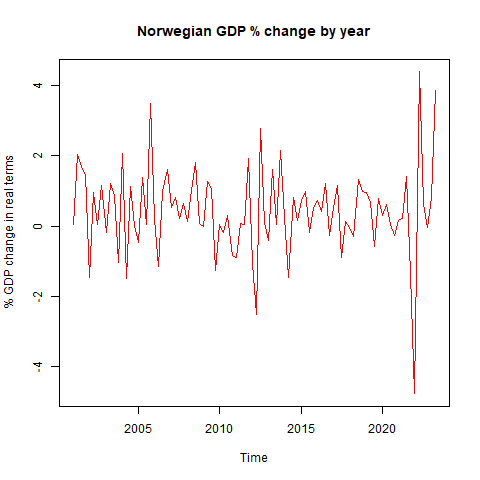
\includegraphics[width=10cm]{gdp.png}
		\centering
		\caption{Norwegian real GDP \% change.}
		\label{fig::gdp}
	\end{figure}
	
	The GDP change is also not normal (S-W $p = 0.0004$, K-W $p = 0.008$), auto-correlated at lags 1 (ACF), and partially auto-correlated (PACF) at lags 1 and 2.
	
	We discover that using a Moving Average model at Lag 1 (MA(1) model) results in no auto-correlations, showing that our data are relatively stable otherwise. This was to be expected, since the time scale these data were collected (yearly quarters) absorbs most of the shocks and time-dependent variance which typically plague other financial time series. Our model can thus be written as such:
	
	$$
	RGDP_t = 0.4166 -0.3455 \epsilon_{t-1}
	$$, where $\epsilon_{t-1}$ are the errors of the previous prediction
	
	Following the Box-Jenkings methodology we confirm that this is the best simple ARIMA model for explaining Norwegian GDP. The resulting residuals are almost normal (S-W $p=7.85e-05$, K-S $p=0.08541$, where we prefer the K-S test, since S-W is a very strong test which tends to always dismiss normality on large datasets) and homogeneous. Homogeneity is challenged at lags 6 and 38, but given their position (very long lags) and their lack of pattern, we can safely dismiss them as noise. We can hypothesize that these variations and deviations from normality are caused primarily by the erratic change of GDP during the COVID period.
	
	
	\section{Predicting GDP based on other factors}
	
	We fit a model with the parameters outlined in Table \ref{tab::params}.
	
	\begin{table}
		\centering
		\rowcolors{2}{gray!25}{white}
		\begin{tabular}
			{ |p{3cm} | p{3cm} | p{5cm}| }
			\hline
			\textbf{Name} & \textbf{Type} & \textbf{Description} \\
			\hline
			LAG\{p\}  & Numeric & Norwegian RDGP \% change for  Lags $p \in 1 \cdots 4$\\
			OIL WTI  & Numeric & World Oil Index \\
			Diff WUI  & Numeric & Quarterly difference of World Uncertainty Index \\
			Diff PI & Numeric & Quarterly difference of Pandemic Index \\
			RPROD NOR  & Numeric & \% change of Norwegian Production Index \\
			CREG NOR  & Numeric & Car Demand Index \\
			DUNEM NOR  & Numeric & Difference of Unemployment Index \\
			PPI  & Numeric & Producer Index \\
			CONPROD  & Numeric & Construction Index \\
			DLONGR NOR  & Numeric & Difference of Long Term Interest Rates\\
			DLONGR NOR  & Numeric & Difference of Long Term Interest Rates\\
			STEXCHNOR & Numeric & Market Index \\
			LEADNOR & Numeric & Leading Indicator \\
			\hline
		\end{tabular}
		\caption{An overview of the data used in our model.}
		\label{tab::params}
	\end{table}
	
	Fitting a model with all the parameters results in normal residuals (S-W $p = 0.1089$, K-S $p=0.6733$), with no multicollinearity, and no homoscedascity (volatility-through-time) problems (L-B for squared errors $p=0.9997$).
	
	Table \ref{tab::gdp_model} shows the final model used for the Norwegian GDP predictions, selected manually by AIC. The model can be written as:
	$$
	RGDP = 0.303 + 0.722 * RPROD + 0.239 * LEAD
	$$
	where the variables are interpreted according to Table \ref{tab::params}.
	
	The model's residuals are normal (K-S $p=0.1477$, L-B $p=0.9781$), with no autocorrelations and constant variance through time (L-B with squared errors $p=1$), with no multicolinearity. The model exhibits an AIC of $207.8$ and $R^2_{adj} = 0.573$.
	
	%
	
% Table created by stargazer v.5.2.3 by Marek Hlavac, Social Policy Institute. E-mail: marek.hlavac at gmail.com
% Date and time: Fri, Nov 03, 2023 - 2:53:02 PM
\begin{table}[!htbp] \centering 
  \caption{Linear regression model predicting real GDP Growth (\%).} 
  \label{tab::gdp_model} 
\begin{tabular}{@{\extracolsep{5pt}}lc} 
\\[-1.8ex]\hline 
\hline \\[-1.8ex] 
 & \multicolumn{1}{c}{\textit{Dependent variable:}} \\ 
\cline{2-2} 
\\[-1.8ex] & `RGDP NOR` \\ 
\hline \\[-1.8ex] 
 `RPROD NOR` & 0.722$^{***}$ \\ 
  & p = 0.000 \\ 
  LEADNOR & 0.239$^{***}$ \\ 
  & p = 0.00004 \\ 
  Constant & 0.303$^{***}$ \\ 
  & p = 0.002 \\ 
 \hline \\[-1.8ex] 
AIC & 207.8 \\ 
Observations & 82 \\ 
R$^{2}$ & 0.584 \\ 
Adjusted R$^{2}$ & 0.573 \\ 
Residual Std. Error & 0.834 (df = 79) \\ 
F Statistic & 55.414$^{***}$ (df = 2; 79) \\ 
\hline 
\hline \\[-1.8ex] 
\textit{Note:}  & \multicolumn{1}{r}{$^{*}$p$<$0.1; $^{**}$p$<$0.05; $^{***}$p$<$0.01} \\ 
\end{tabular} 
\end{table} 

	%
	
	
	
	
	
\end{document}